
\section{Introduction}
\label{section:intro}
VI =================
check if double quotes are in the right direction
================== VI
In this report, we will provide the results of a careful investigation of the performance of a variety of software packages applied to a typical initial value ordinary differential problem encountered in Covid-19 modeling. 

For any mathematical model, the accuracy requirements of the numerical solution should be determined by the quality of the model and the accuracy of the parameters that appear in the model. Numerical errors associated with the computational techniques that are used to obtain the solution must always be negligible compared to the accuracy to which the model is defined. \emph{Researchers deserve to obtain numerically accurate solutions to the models that they are studying}. In this report, \emph{we will show that the straightforward use of standard IVODE solvers on typical Covid-19 models can lead to numerical solutions that have large errors, some of the same order of magnitude as the solution itself.}

In Section $\ref{subsection:research_papers}$, we review examples of how Initial Value Ordinary Differential Equation Solvers (IVODES) are used in epidemiology. In Section $\ref{subsection:SEIR_model}$, we define the SEIR models which we will consider throughout this report, in Section $\ref{subsection:exponential_growth}$, we discuss the problem of stability as it concerns problems with exponential growth, in Section $\ref{subsection:fixed_vs_control}$, we explain the difference between fixed step-size and error-controlled solvers. The IVODE software packages from programming environments that are typically used by researchers are described in Section $\ref{subsection:numerical_software_used}$. We also make a note of issues with evaluation at output points that lead to inefficiencies in Section $\ref{subsection:solution_output_points_impl}$. In Section $\ref{subsection:effect_of_discontinuity}$, we discuss the effects of problem discontinuities on the performance of these solvers.

In Section $\ref{subsection:naive_time_problem}$, we apply the solvers to the problem with a time-dependent discontinuity and show how this results in numerical solutions with relative errors of the same magnitude as the solution we are trying to compute. In Section $\ref{subsection:time_disc_handling}$, we will use discontinuity handling to solve the time-dependent problem. In Section $\ref{subsection:time_tolerance_study}$, we will use a range of tolerances to discuss the effects of tolerance on the accuracy and efficiency of the solvers.

In Section $\ref{subsection:naive_state_problem}$, we apply the solvers to the Covid19 problem with a state-dependent discontinuity and show how none of the solvers were able to obtain accurate solutions. We will explain how even the use of very sharp tolerances does nothing to improve the models in Section $\ref{subsection:state_sharp_tol_failed}$ and show that the only proper way to solve this problem is through event detection, which we will describe in Section $\ref{subsection:intro_event_detection}$. We then show the correct solution to the problem in Section $\ref{subsection:state_with_event_detection}$ and perform a tolerance study on this problem in Section $\ref{subsection:state_tolerance_study}$.

In Section $\ref{section:fortran_inaccuracies}$, we examine the implementation details for some of the solvers to investigate the cause of the inaccuracies. We conclude the report in Section $\ref{section:summary}$ with a summary and the identification potential for future work projects.

\subsection{Epidemiological modelling}
\label{subsection:research_papers}
One common form of an epidemiological study is forecasting. Using previously obtained parameters, the researcher develops a mathematical model involving differential equations which are solved using an ODE solver. Often, the solver will be used to integrate over a large time period so that the researcher can examine how the diseases will spread. For such problems, sharp tolerance values should be used and the solver-problem combination is expected to be resilient over large time periods. In Section $\ref{subsection:exponential_growth}$, we discuss why it is unrealistic to attempt to compute a numerical solution for large time periods if the infection is still growing exponentially but how measures such as social distancing allow solvers to reduce modeling errors so reasonably accurate solutions can be computed over longer time periods.

A second type of epidemiology study involves parameter estimation. In this kind of study, data points are collected about the spread of a virus and we try to fit a mathematical model through that data. In so doing, we can estimate the parameters used by looking at which parameters minimize the error in the fit. The parameters estimated can tell us if implemented control measures are working and may point out what can be done to improve the situation. An example of such a study can be found in Section $\ref{section:ebola_paper}$. Also, parameters so estimated can be used for the first kind of study. Parameter estimation studies often involve using an ODE solver inside some optimization algorithm and thus the computing time, especially with large problems, can be significant. We will therefore investigate whether or not researchers can coarsen the tolerance.

\subsection{Detailed description of two specific models to be considered in this report.} 
\label{subsection:SEIR_model}
In this section, we explain how an IVODE problem is defined. We then (Reference Christina Christara.) describe the models that we are going to consider in this report. They involve typical SEIR models to which we add discontinuities.

An IVODE problem is defined with:
\begin{equation}
y'(t) = f(t, y(t)), y(t_0) = y_0 \nonumber
\end{equation}
where f is a function that defines the derivative at that that point in time, t. A complete definition also includes the initial value of the solution. Thus given $y'(t)$ and $y(t_0)$, we find $y(t)$ using numerically methods. 

To fulfill the complete problem definition, we define as models as follows:
\begin{equation}
\frac{\textit{d}S}{\textit{dt}} = \mu N - \mu S - \frac{\beta}{N}IS, \nonumber
\end{equation}

\begin{equation}
\frac{\textit{d}E}{\textit{dt}} = \frac{\beta}{N}IS - \alpha E - \mu E, \nonumber
\end{equation}

\begin{equation}
\frac{\textit{d}I}{\textit{dt}} = \alpha E - \gamma I - \mu I, \nonumber
\end{equation}

\begin{equation}
\frac{\textit{d}R}{\textit{dt}} = \gamma I - \mu R, \nonumber
\end{equation} 

In this SEIR model, we describe the epidemic over time. S is the number of susceptible individuals, E is the number of exposed individuals, I is the number of infected individuals and R is the number of recovered individuals at a point in time. We also use N to represent the population size.
The other parameters in this model are as follows: $\alpha$ is such that $\alpha^{-1}$ is the average incubation period, $\beta$ is the transmission rate, $\gamma$ is the recovery rate and $\mu$ is the replenishment rate. In this report, we assume that all these parameters are known as our goal is to investigate the performance of IVODE solvers on the test problems. We will see that we get solutions that are not efficiently computed or that may have significant errors. This issue can have serious consequences as it will fail to show the actual impact of the virus as it corresponds to the actual epidemiology theories behind the mathematical models. These incorrect numerical solutions may lead epidemiologists into reaching incorrect conclusions and thus lead them to try to change the mathematical models themselves when, in fact, it is the solvers which are at fault.

The discontinuities we are going to consider involve the parameter $\beta$.
Before measures such as social distancing and others are implemented, $\beta$ has a much higher value than after. In our case, $\beta$ will be 0.9 before the measures and 0.005 after they are implemented. Such an abrupt change in a modeling parameter introduces a discontinuity as we will show in Section $\ref{subsection:effect_of_discontinuity}$. 

For the time-dependent discontinuity, we will assume that at some point in time, measures are implemented that will lead to a reduction in the parameter $\beta$. We would like to model the problem through this discontinuity but as we will show, this discontinuity introduces a numerical issue.

For the state-dependent discontinuity, we consider the following situation. If the population of exposed people reaches a certain maximum threshold, measures are introduced, which decreases the value of $\beta$. This introduces a discontinuity. Then, when the population of exposed people drops below a certain minimum threshold, the measures are relaxed, which increases $\beta$ back to its original value, which introduces another discontinuity. We will try to model this problem through a long time period corresponding to `waves' of the pandemic. We note that each time we change the parameter $\beta$, a discontinuity is introduced and thus this problem is far more discontinuous than the previous one, which had only one discontinuity. In so doing, we show that all the solvers will fail.

The other parameters are assumed to always be constant with N at 37,741,000 (the approximate Canadian population size), $\alpha$ at 1/8, $\gamma$ at 0.06, and $\mu$ at 0.01/365.

The initial values are E(0) = 103, I(0) = 1, R(0) = 0 and S(0) = N - E(0) - I(0) - R(0).

This gives us a complete system of initial value ordinary differential equations that is in a form that can be solved by typical software packages.

\subsection{Exponential growth and the issue of instability}
\label{subsection:exponential_growth}
It turns out that some of the solution's components to the SEIR model exhibit exponential growth over certain time periods. In this section, we discuss exponential growth and its impact on the computation of a numerical solution. First of all, we give a quick overview of stability for ODEs. Then we will show that the SEIR model is unstable and how measures such as social distancing can improve the stability. This is important as this essentially means that before measures are implemented, accurate models are for the most part very difficult to obtain but the addition of the measures such as social distancing can give us hope that the solvers will perform better.

The stability of an ODE is associated with the impact of small changes to the initial values on the solution to the problem. An ODE is unstable if a small change in the initial values results in drastically different solutions; otherwise, the ODE is said to be stable.

It is straightforward to see that the solution to problems that exhibit exponential growth are unstable. This is the case with some of the solution components of a Covid-19 model. The population of infected people grows exponentially for as long as there are no measures. This means that ODE solvers will experience difficulties in obtaining accurate numerical solutions. 

In Figure $\ref{fig:unstability_of_exponential_growth}$, we show exponentially growing solutions corresponding to models with slightly different initial value of E(0). We can see that we get different solutions, that become even more different as time increases.

\begin{figure}[h]
\centering
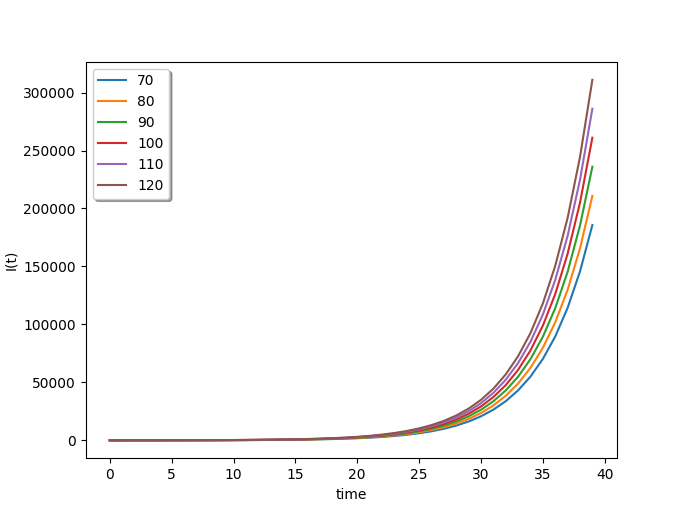
\includegraphics[width=0.7\linewidth]{./figures/unstability_of_exponential_growth}
\caption{Instability of exponential growth}
\label{fig:unstability_of_exponential_growth}
\end{figure}

However, when we introduce measures such as social distancing, which leads to a smaller $\beta$ value, the problem will exhibit slower exponential growth or can even show exponential decay. A slower exponential growth means that the solution will not be as sensitive to changes to the initial values. Exponential decay is even better as the solutions from different initial values will converge.

Epidemic modeling problems exhibit solutions with this type of behavior. At first, the problem is unstable but as measures are implemented, which lead to exponential decay rather than growth, the problem becomes stable. We show this in Figure $\ref{fig:regain_stability_after_measures}$ for the problem with the time-dependent discontinuity. At first, the solutions diverge during exponential growth, but the addition of measures such as social distancing introduce exponential decay which makes them converge. Thus the measures not only save lives but also improve the accuracy of the computed solutions.

\begin{figure}[h]
\centering
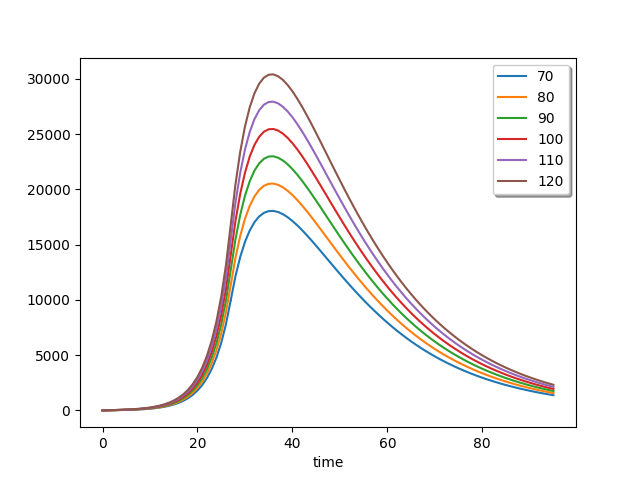
\includegraphics[width=0.7\linewidth]{./figures/regain_stability_after_measures}
\caption{Unstable solutions in the region [0, 40] gain in stability as measures are implemented in the region [40. 90]}
\label{fig:regain_stability_after_measures}
\end{figure}

\subsection{Brief overview of numerical software to be employed in the numerical solution of this model}
We start by explaining how solvers attempt to solve an IVODE problem. Given the values at the initial time, $t_0$, the solver will use an initial step size, $h$, to compute a solution at time, $t_1 (= t_0 + h)$. Similarly, the solvers will attempt to take a sequence of steps until it reaches the end time. High-quality solvers will then run an interpolation algorithm either locally within each step or globally across the sequence of points to get the numerical solution. We note that a solver is said to have order, $p$ if the difference between the actual solution and the computed solution is equal to $O(h^p)$

In the next section, we describe what a solver will attempt to do to improve the accuracy of their solutions. We then discuss the numerical solvers we are going to use throughout our investigation. We will then have an additional discussion on the implementation of the interpolation to get the final solution and how certain programming environments have not updated their solvers to use interpolation.

\subsubsection{Fixed Step Size and Error Control Solvers}
\label{subsection:fixed_vs_control}
We begin our discussion on the software used by giving a brief overview of what role is played by the tolerance and the difference between fixed step size and adaptive step-size error control solvers.

The tolerance is a measure of how accurate we want the solution computed by the solvers to be. Generally, an absolute tolerance of $10^{i}$ means that we want the error estimate to be within $10^{i}$ whereas a relative tolerance of $10^{i}$ means that we want the ratio of the error estimate and the computed solution to be within $10^{i}$. This is not always the case as some solvers will make a blended use of the provided absolute and relative tolerance.

A solver is said to have a fixed step size if it does not compute an error estimate that can be compared to the tolerance. The solver will have an initial step-size and this step-size is used throughout the whole integration. It will jump from one point to another point in a 'step' and will not check if the numerical solution it obtains at the end of the step is sufficiently accurate. Thus, the distance between the points, i.e the step size, is constant throughout the computation.

An error controlled solver starts with an initial step size but as it takes a step, it will compute an error estimate and based on the tolerance will repeat the computation with a smaller step-size if the error estimate is larger than the tolerance. It will repeat the process until the error estimate satisfies the given tolerance. Only then will it move to the next step. Thus it reduces the step-size to step throughout the computation. Also, if the error estimate is much smaller than the tolerance, it will increase the step-size for the next step. This allows it to make sure that the given tolerance is satisfied over the whole problem interval and that as large a step as possible is being taken to optimize the efficiency of the computation.

Error control is not simple to implement. This is where we need to caution against the use of non-standard ODE solvers or fixed step-size solvers. Also, some researchers, who have some understanding of ODEs may be tempted to write their solvers. These researchers often program a non-error control method like a simple fixed step-size Euler or Runge-Kutta method. We will show, using provided fixed step-size solvers in R, how these solvers simply cannot solve a Covid-19 model. Without error control, these solvers cannot handle the discontinuity and stability issues that are present in these models and they will give very erroneous solutions, often without even a warning that the computed solutions should not be trusted.

\subsubsection{The packages}
\label{subsection:numerical_software_used}
There are different types of ODE solvers that are grouped in the following classes: Runge-Kutta methods, Runge-Kutta pairs, and multi-step methods.

A Runge-Kutta method is a one-step method using function evaluations along the step. It integrates with a sequence of steps and has no error control. An example is the classical Runge-Kutta method.

A Runge-Kutta pair is a solver that uses two Runge-Kutta methods. One of the methods is used to compute a solution and a second method is used to compute an error estimate. The then resize the step based on that error as discussed previously. An example is the DOPRI5 pair that uses a fifth-order method for the solution and a fourth-order method for the error estimate.

a multi-step method is a solver that will use a linear combination of the previous step to take the next step. An example is LSODA.


\subparagraph{R packages}
Scientists who solve ODE models in R commonly use the deSolve package and the $ode()$ function within it.
$ode()$ provides many numerical methods to solve a problem but we have focused our investigation only on the following popular choices: `lsoda', `daspk', `euler', `rk4', `ode45', `radau', `bdf' and `adams'. The default method is `lsoda' and the default tolerances are $10^{-6}$ for both the absolute and relative tolerances. We also note that we did not consider the other integrators in the deSolve package like $rkMethod()$, which present other Runge-Kutta methods, and the other ones which are called by the $ode()$ function itself.

The error control methods solvers are:
\begin{itemize}
\item Using `lsoda' calls the Fortran LSODA routine from ODEPACK. It can automatically detect stiffness and choose between a stiff and a non-stiff solver.
\item Using `daspk' calls the Fortran DAE solver of the same name.
\item Using `ode45' calls an implementation of Dormand-Prince (4)5 (DOPRI5), written in Fortran. We note that it is not using DOPRI5.f.
\item Using `radau' calls the Fortran solver RADAU5 which implements the 3-stage RADAU IIA method.
\item Using `bdf' calls the stiff solver inside the Fortran LSODE package which is based on a family of BDF (Backward Differentiation) methods.
\item Using `adams' calls the non-stiff solver inside the Fortran LSODE package which is based on a family of Adam's methods.
\end{itemize}

The fixed step-size solvers are:
\begin{itemize}
\item `euler' which calls the classical Euler method which is implemented in C.
\item `rk4' which uses the classical Runge-Kutta method of order 4 which is implemented in C. 
\end{itemize}

We will use these two methods to demonstrate what happens when researchers program their non-error-controlled solvers.

We also make note that R uses a dubious method to find the values of the solution at output points. This results in efficiency issues as we will discuss in Section $\ref{subsection:solution_output_points_impl}$. 

We next talk about the R's interface, the `ode' function is only given a vector of the output points. The function decides itself when to use interpolation or stopping at output points as described in Section $\ref{subsection:solution_output_points_impl}$. There are ways to use interpolation explicitly but Researchers will have to dive into the documenting papers/source code to find it. 

\subparagraph{Python packages}
In Python, researchers use the scipy.integrate package and will normally use the $solve\_ivp()$ function due to its newer interface. It lets the user apply the following methods: `RK45', `RK23', `Radau', `BDF', `LSODA' and 'DOP853`. In this report, we will investigate all of these methods. The default solver in $solve\_ivp()$ is `RK45' and the default tolerance is $10^{-3}$ for the relative tolerance and $10^{-6}$ for the absolute tolerance. All of these solvers employ some form of error control. 

\begin{itemize}
\item Using `RK23' uses an explicit Runge-Kutta pair of order 3(2). This uses the Bogacki-Shampine pair of formulas. It is a Python implementation.
\item Using `RK45' uses an explicit Runge-Kutta pair of order 5(4). This uses the Dormand-Prince pair of formulas. It is a Python implementation.
\item Using `DOP853 uses an explicit Runge-Kutta pair of order 8. It is a Python implementation.
\item Using `Radau' uses an implicit Runge-Kutta method, the three-stage Radau IIA method of order 5. It is a Python implementation.
\item Using `BDF' uses a method based on backward-differentiation formulas. This is a variable order method with the order varying automatically from 1 to 5. It is a Python implementation.
\item Using `LSODA' calls the Fortran ODEPACK for LSODA. This switches between an Adams (non-stiff) and a BDF (stiff) method as it detects stiffness. This is implemented in Fortran.
\end{itemize}

We note that all solvers in $solve\_ivp()$ have error control and that only 'LSODA' is using the Fortran package itself, the others are a Python implementation and will likely be slower.

We next talk about Python's $solve\_ivp()$ interface. It can integrate using only the initial time and the final time where it will return the output points where the steps stopped. It can also take a $t\_eval$ vector which does local interpolation. It lets the solver take as big a step as it can and does not force the solver to stop at the output points. Thus it does not suffer from the inefficiencies described in Section $\ref{subsection:solution_output_points_impl}$. The interface also has a $dense\_output$ flag. This returns an interpolation on the whole time range and allows the user to use the result as a function.

\subparagraph{Scilab packages}
In Scilab, researchers solve differential equations with the built-in $ode()$ function which has the following methods: `lsoda', `adams', `stiff', `rk', `rkf'. The default integrator is `lsoda'.
Default values for the tolerances are respectively $10^{-5}$ for the relative tolerance and $10^{-7}$ for the absolute tolerance for all solvers used except `rkf' for which the relative tolerance is $10^{-3}$ and the absolute tolerance is $10^{-4}$. All of these solvers are error control solvers.

\begin{itemize}
\item Using `lsoda' will call the Fortran LSODA code from ODEPACK. This switches between an Adams (nonstiff) and a BDF (stiff) method as it detects stiffness. It has error control.
\item Using `stiff' calls the stiff solver inside Fortran's LSODE package which is based on a family of BDF (Backward Differentiation) methods.
\item Using `adams' calls the non-stiff solver inside the Fortran LSODE package which is based on a family of Adam's methods.
\item Using `rk' calls an adaptive Runge-Kutta method of order 4. It uses Richardson extrapolation for the error estimation. It is implemented in Fortran in a program called 'rkqc.f'.
\item Using `rkf' calls the Shampine and Watts program based on Fehlberg's Runge-Kutta pair of order 4 and 5 (RKF45) pair. It calls the Fortran rkf45.f.
\end{itemize}

We next talk about the $ode()$ interface in Scilab. It takes a vector of time steps and the code decides whether to use interpolation or to stop the integration at the output points as described in $\ref{subsection:solution_output_points_impl}$. We note that Scilab's `rkf' is a very old software package that it does not even have interpolation.

\subparagraph{Matlab packages}
In Matlab, researchers solve differential equations with the built-in $ode()$ family of functions. We will consider two of those in $ode45$ and $ode15s$.
Default values for the tolerances are respectively $10^{-3}$ for the relative tolerance and $10^{-6}$ for the absolute tolerance for all solvers as they all use the $odeset options$.

\begin{itemize}
\item Using $ode45$ calls a Matlab implementation of DOPRI5.
\item Using $ode15s$ employs an algorithm that is a variable-step, variable-order (VSVO) solver based on the numerical differentiation formulas (NDFs) of orders 1 to 5. Optionally, it can use the backward differentiation formulas (BDFs, also known as Gear's method) that are usually less efficient. It is a stiff ODE solver.
\end{itemize}

We next talk about Matlab's ode suite's interface. The interface takes the initial and final time only and allows the solvers to take as big a step as it needs. All plots are then done using interpolation by the plotting software so it does not suffer from the issues discussed in Section $\ref{subsection:solution_output_points_impl}$

\subparagraph{How the packages relate}
We tried to find connections across the programming environment where the solvers appear to be using the same source codes.
Here is what we found:

R's, Python's, and Scilab's `lsoda' are all wrappers around the Fortran LSODA code inside ODEPACK.

R's `bdf' is equivalent to Scilab's `stiff' in that they use the LSODE code inside ODEPACK but Python's "BDF" is a different implementation in Python itself.

Matlab's $ode15s$ was not set to using BDF.

R's `adams' and Scilab's `adams' are similar in that they both use the LSODE code from ODEPACK.

R's and Python's Runge Kutta 4(5) pairs are both implementations of DOPRI5 but they have different source code as Python implements its own. R does not use the DOPRI5.f file. Scilab's `rkf' is not the same pair as it is using the Shampine and Watts Fehlberg's Runge-Kutta pair, not the Dormand-Prince pair. $ode45$ in Matlab is a Matlab implementation of DOPRI5.

Scilab's `rk' which is of order 4 and R's `rk4' are not the same solvers. Scilab's `rk' is adaptive (error-controlled with Richardson extrapolation for the error estimate) whereas R's `rk4' is a fixed step-size method.

R's `Radau' and Python's `Radau' have different source codes as Python implements its own `Radau' code while R appears to be called the Fortran code for Radau5.

\subsection{Observation on obtaining solution approximations at output points}
\label{subsection:solution_output_points_impl}
VI ===================
Include paragraph on interpolation
=================== VI

In this section, we discuss an issue that we encountered with some of the ODE solvers in R and Scilab when it comes to plotting. In an ideal scenario, the user's desired output points should not interfere with the efficiency of the solvers. However, in these two platforms, an old method for outputting is used which makes asking for a lot of output points very inefficient.

Normally, an ODE solver will work as follows: it will have a default initial step-size, will take a step, and will then adjust the step-size based on the error estimate associated with the solution approximation for the given step and then it will use this new step-size to take the next step. This process is repeated until the solver reaches the end of the interval. However, often the users of an ODE solver will require outputs at specific points and these points may lie at points that are internal to the steps. The current state-of-the-art approach to get solution approximations of these output points is to perform a high accuracy interpolation on the given step and to return the value of that interpolant at the required point. The accuracy of the interpolation on new solvers is at least of order $p$ if the numerical ODE solution is of order $p$.

In R and Scilab, this new method is not used in all the solvers. Instead, R and Scilab will use the output points to dictate the step-size. This issue arises when many output points appear before the steps that would normally be taken by the solver. These solvers will thus use an initial step size or the difference between the start point and the next output point as the initial step-size and step to this next point. The solver will then repeat the process between each consecutive pair of output points. Thus the space between points will limit the maximum step-size that can be taken and will lead to additional function evaluations because the solver needs to pause at each output point. This will lead to a considerable drop in efficiency as we will show, for instance in Tables $\ref{tab:tolerance_time_discontinuity_rk45_R}$ and $\ref{tab:tolerance_time_discontinuity_rk45_further_R}$. These tables show that a problem that can be solved with 150 function evaluations will be solved with 500 function evaluations when there are many outputs. This increase in the number of function evaluations will correspond to increases in CPU time. 

This old method of implementing output points also means that the accuracy of the solution depends on the space between the output points. Both in an error-control and a fixed step-size solver, the step-size in this interval will be the maximum of the difference between two output points. Thus, we get the unusual behavior that the accuracy is increased by putting the points closer together and the accuracy is decreased by putting them further apart. We will point out these inconsistencies as they become relevant later in this report. We also note that spacing the points closer together is not a good way to control the accuracy as no researcher will know beforehand how close the points should be.

\begin{figure}[h]
\centering
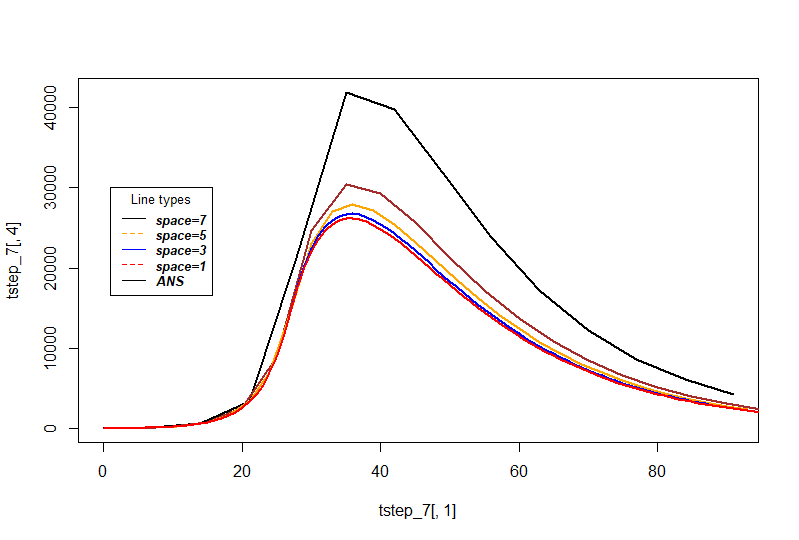
\includegraphics[width=0.7\linewidth]{./figures/R_ode45_spacing_experiment}
\caption{R `ode45' spacing between points experiment}
\label{fig:ode45_spacing_experiment}
\end{figure}

Figure $\ref{fig:ode45_spacing_experiment}$ shows an experiment where we solve an ODE problem using R's 'ode45', which is an implementation of DOPRI5 which has error control but is not using interpolation, to show that it is doing more function evaluation than needed. We set both the absolute and relative tolerance to 0.1 and thus expect low accuracy but very good efficiency. However, the space between the points is still a limiting factor for the step-size and the solution is somewhat accurate although very inefficient. We recorded the number of function evaluations in Table $\ref{tab:ode45_spacing_experiment}$ and it can be seen that R is using a lot more function evaluations than are needed to satisfy such coarse tolerances.

\begin{table}[h]
\caption {R DOPRI5 spacing experiment} \label{tab:ode45_spacing_experiment} 
\begin{center}
\begin{tabular}{ c c }
spacing & nfev \\ 
1 & 572 \\
3 & 188 \\
5 & 116 \\
7 & 80 \\
\end{tabular}
\end{center}
\end{table}

From Figure $\ref{fig:ode45_spacing_experiment}$ and Table $\ref{tab:ode45_spacing_experiment}$, we note that we did not ask the solver for an accurate solution and that it is giving us an excessively accurate solution. This excess accuracy comes at a price of around 500 more function evaluations. Accuracy should ideally be completely determined by the tolerance but using this old method for dealing with output points substantially interferes with this ideal. This results in the solver not being allowed to take as big a step as that should be based on the tolerance, and this leads to substantial inefficiency. 

We advise users to use interpolation software whenever readily available so that the solvers can run as efficiently as possible. When faster CPU times are required, the researcher can look to see if their chosen solver is using interpolation or if it is taking unnecessary steps. If their chosen solver is using the old method, we advise using a different solver that has an internal interpolant whenever possible or running their solvers with an appropriately spaced out set of points and running an interpolation on the output to obtain a smooth plot of the solution. We also reiterate that the interpolant should be at least of order $p$ if the ODE solver gives a solution of order $p$ so that the interpolation error does not interfere with the solution more than the ODE error.

\subsection{Discontinuities and their effects on solvers}
\label{subsection:effect_of_discontinuity}
The main purpose of this report is to discuss how to model discontinuities and how these affect the process of computing a numerical solution to the model. In this section, we will show what happens when a solver meets a discontinuity and how this leads to erroneous solutions.

We need to understand that all the solvers use numerical methods based on Taylor series, one of the core assumptions of which is that the function and all its relevant derivatives are continuous. If the right-hand side function is discontinuous, this theory no longer holds and the solvers are no longer guaranteed to converge to the actual solution as the step-size goes to 0.

We will see that discontinuities will have huge impacts on the efficiency of the solvers, that some solvers, even with error control, will require an extremely sharp tolerance to step over the discontinuity, and that fixed-step solvers simply cannot solve these problems accurately. 

It is important to note that the step that first meets a discontinuity will almost always fail. This is because for the code to step over a discontinuity, the step size needs to be much smaller than the one that is being used before the discontinuity. The codes will thus have to retake the step with smaller step size and as long as the error estimate is not small enough, it will need to continue reducing the step. This leads to high numbers of function evaluations near the discontinuity which will lead to longer CPU times. 

\begin{figure}[h]
\centering
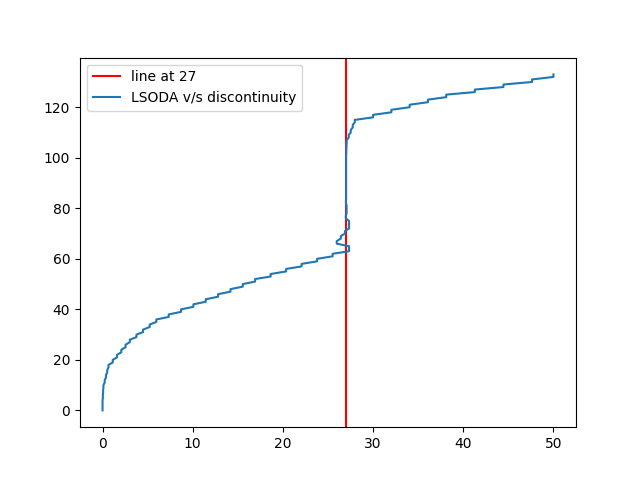
\includegraphics[width=0.7\linewidth]{./figures/lsoda_vs_discontinuity}
\caption{Function evaluations for `LSODA' when there is a discontinuity at t=27}
\label{fig:lsoda_vs_discontinuity}
\end{figure}

\begin{figure}[h]
\centering
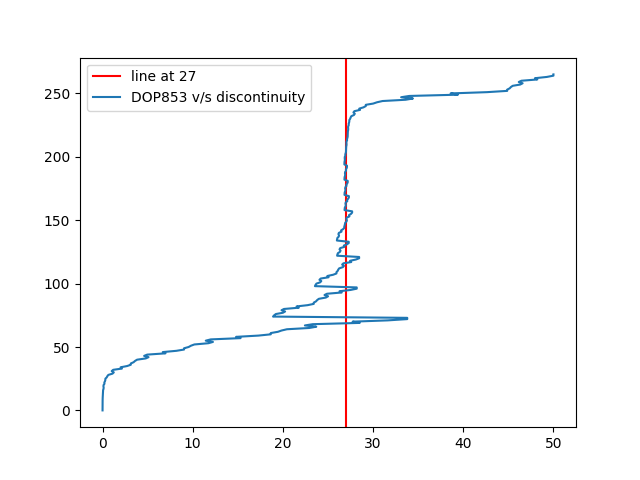
\includegraphics[width=0.7\linewidth]{./figures/dop853_vs_discontinuity}
\caption{Function evaluations for `DOP853' when there is a discontinuity at t=27}
\label{fig:dop853_vs_discontinuity}
\end{figure}

In Figures $\ref{fig:lsoda_vs_discontinuity}$ and $\ref{fig:dop853_vs_discontinuity}$, we run `LSODA' and `DOP853' from Python on a discontinuous problem where the discontinuity is introduced at time 27 and plot the time at which the $i^{th}$ function evaluation occurs. We thus show the spike in the number of function evaluations at the discontinuity as the solvers repeatedly retake that step with smaller and smaller step-sizes.

Following this discussion, we also recommend epidemiologists carry out a manual discontinuity detection experiment to see if their model has any discontinuity. This trivial experiment is done by collecting at what time the solver made the $i^{th}$ call to the solver. The pseudo-code of which is as shown below:

\begin{minipage}{\linewidth}
\begin{lstlisting}[language=Python]
times = []
function_calls = []
count = 0

function model(t, y)
    global times, function_calls, count
    times.append(t)
    function_calls.append(count)
    count += 1 

    // code to find the derivatives
    return <derivatives>

plot(times, function_calls)
\end{lstlisting}
\end{minipage}

In the experiment outlined in this pseudo-code, we plot the time against the cumulative count of the function calls. An almost straight vertical line on this graph will indicate that the function was called repeatedly at a specific time and thus that the solver repeatedly changed the step-size in this region to step over a discontinuity. Thus the epidemiologist can detect a discontinuity and can perform further tests. In the remainder of this report, we will outline the ways to accurately and efficiently solve problems with such discontinuities.


